\documentclass{article}

% MATH-AI 2026 (The 6th Workshop on Mathematical Reasoning and AI, NeurIPS
% 2026, Atlanta). 4-page main body, NeurIPS 2026 workshop format, unlimited
% references, trimmed appendix. Double-blind, per the CFP: anonymous author
% block, no identifying URLs, prior work cited in third person. Add ",final"
% at camera-ready (which allows 5 body pages).
\usepackage[dblblindworkshop]{neurips_2026}
\workshoptitle{The 6th Workshop on Mathematical Reasoning and AI (MATH-AI)}

\usepackage[utf8]{inputenc}
\usepackage[T1]{fontenc}
\usepackage{hyperref}
\usepackage{url}
\usepackage{booktabs}
\usepackage{array}
\usepackage{amsfonts}
\usepackage{nicefrac}
\usepackage{microtype}
\usepackage{graphicx}
\usepackage{xcolor}
\usepackage{float}   % [H]: pin Table 1 under its own heading, never float it away
\usepackage{macros}

\graphicspath{{figures/}}

\title{A Proof Attempt Told the Search Where to Look:\\
A Case Study in Machine-Assisted Mathematical Research}

\author{%
  Anonymous Author(s) \\
  Affiliation \\
  Address \\
  \texttt{email} \\
}

\begin{document}

\maketitle

\begin{abstract}
We report a research loop in which a numerical search and a human proof
attempt corrected each other, in enough detail that the mechanism is
visible. An adversarial machine search over experimental designs suggested
that a certain estimation-theoretic lower bound could not be beaten even by
an adversary who knows the model's functional form. The best ratio it found
after thousands of designs was $1.005$, so we wrote the bound down as
structure-proof. The proof we then wrote did not cover that claim. It
established the bound only within two curvature lengths of the anchor point,
and the obstruction was a single inequality that fails outside that region.
Searching exactly where the proof stopped produced a counterexample: a
four-point design with one far probe of weight $3\times 10^{-4}$, attaining
ratio $0.8517$, verified at 50-digit precision. The earlier verdict was a
search artifact, and the result is now two-sided and exact. Neither half of
the loop found this alone. We place the episode inside a larger body of
machine-checked mathematics on the cost of self-knowledge in performative
prediction, in which eleven measurement-forced pivots are recorded in the
code where each occurred.
\end{abstract}

\section{Introduction}
\label{sec:intro}

This paper is about how a piece of mathematics got made, and it uses one
concrete body of theory as the specimen. Our answer to the venue's guiding
question is narrow and, we hope, checkable. In the loop we ran, machines were
good at refuting and at certifying, people were good at proving, and the
interesting events happened where the two disagreed. We document one such
event completely, then ask how far it generalizes using ten more of its own
kind.

The specimen is a theory of what it costs a decision-maker to learn how its
own deployed actions reshape the world it then retrains on. Section
\ref{sec:substrate} says what that means in plain terms. What matters here is
that the theory is large enough to have a texture: proved theorems,
numerically supported conjectures, and a live simulation pipeline, each of
which turned out capable of correcting the others. Over its development,
measurement forced eleven changes to claims that had already been written
down, and each pivot is recorded in the code file where it happened.

We lead with the eleventh, because it is the one where the two halves of the
loop needed each other. A machine search believed a statement. A human proof
attempt failed to reach the statement, and failed in a way that named the
exact region where it stopped. A second machine search, aimed only at that
region, refuted the statement.

\textbf{What this paper is not.} It is not an autonomous mathematical agent,
and we make no claim in that direction. The proofs here were written by
people. What was automated is numerical checking against declared tolerances,
adversarial search over designs, and high-precision verification of candidate
witnesses. Section \ref{sec:loop} draws that line explicitly.

\textbf{Contributions.}
\begin{enumerate}\itemsep1pt\topsep2pt\parsep0pt
\item A reproducible account of one proof-and-search correction cycle, from
the false belief through the failed proof to the frozen counterexample
(Section \ref{sec:t9}). The resulting statement, Theorem \ref{thm:reach}, is
two-sided and exact.
\item Ten further measurement-forced pivots from the same project, three of
them the same pattern at smaller scale, and an account of what that sample
does and does not support (Section \ref{sec:loop}).
\item The infrastructure that made the correction detectable: a theorem
register carrying per-result proof status, preregistered numerical checks
with tolerances declared before the run, and continuous integration over the
derivation suite (Section \ref{sec:loop}), all shipped as an anonymized
repository in the supplementary material.
\end{enumerate}

\section{The mathematical substrate, briefly}
\label{sec:substrate}

This section says what the theory is about, so that the counterexample in
Section \ref{sec:t9} has something to be a counterexample to. A reader who
wants only the case study can take Theorem \ref{thm:exchange} on faith.

Consider a decision-maker whose deployed action changes the data it will
later retrain on. A dealer who quotes a wide spread sees different order flow
than one who quotes a tight spread, so the flow it must price is partly its
own doing. This is performative prediction
\citep{perdomo2020performative,hardt2023performative}: retraining becomes a
fixed-point iteration, and it converges to a point that is not the one
maximizing value. Algorithms that close that gap
\citep{izzo2021learn,miller2021outside,drusvyatskiy2022stochastic} all need
an estimate of how the distribution responds to the action, and they get it
by perturbing deployments. Those perturbations are deployments of a real
decision variable, so their cost lands in the decision-maker's own objective.

Write $h$ for the scalar action, $\hstar$ for the operating point the
decision-maker would choose if it already knew everything, and
$\dev_t = h_t - \hstar$ for the deviation deployed at round $t$. Let $\eps$
be the response slope to be estimated, $\sigma^2$ the observation noise
variance, $\Phi$ the value function, and $\gpo$ its curvature at $\hstar$.
The cost of exploring is the value forgone,
$C_T = \sum_{t \le T}\E[\Phi(\hstar) - \Phi(h_t)]$. Formal statements are in
Appendix \ref{app:statements}.

\begin{theorem}[Exchange rate; T2]
\label{thm:exchange}
Along any stationary exploration policy, for the least-squares slope
estimator,
$\Var(\hat\eps)\times C_T = \tfrac{1}{2}\gpo\sigma^2\,(1 + o(1))$,
independent of the exploration amplitude, shape, schedule, and of how
strongly the loop contracts.
\end{theorem}

Learning how your own deployment moves the world costs a fixed amount. You
can choose what to buy with it, but not how much to pay. The mechanism is a
cancellation. Information accumulates as the centered energy of the design,
cost accumulates as half the curvature times that same energy, and for
mean-centered exploration the two coincide.

Three further results sit around that identity, all in Appendix
\ref{app:statements}. No policy at all can beat the product, only match it
(T3, T4). The cheapest way to spend a multidimensional budget is to probe
where the objective is flat (T5a, C5.1). And a deployed agent can be made to
correct only when a confidence sequence certifies that correcting cannot
destabilize the retraining loop (L4, P7.1). The theory was also instantiated
on a calibrated real-data problem and on a second economy, both in Table
\ref{tab:results}.

\section{The lead story: a belief, a proof that missed it, and a witness}
\label{sec:t9}

Theorem \ref{thm:exchange} is a statement about one estimator on one class of
policies, and the minimax floors T3 and T4 extend it to all policies and
all estimators. Both leave a natural question open. Suppose the adversary knows
the functional form of the response, not just its slope. Concretely, suppose
it knows that the response is $\tau_\theta(h) = C_0 + C_1 e^{-ch}$ and has
only to learn the three parameters. Knowing the form is real information, so
it might buy a design that beats the floor. Does it?

\textbf{The machine's answer, and why we believed it.} We asked a search. For
each candidate design $\mu$ the relevant quantity is the Cram\'er--Rao
product normalized by the floor,
$R(\mu) = (g^\top M(\mu)^{-1} g)\int (h-\hstar)^2 d\mu$, where $M(\mu)$ is
the design's Fisher information and $g$ is the gradient of the estimand. The
floor survives structural knowledge exactly when $R(\mu)\ge 1$ for every
$\mu$. Four thousand random designs plus 2,500 local refinements returned a
minimum of $R = 1.0050$, and a systematic scan over designs pairing two
near-anchor points with one distant probe found distant probes monotonically
worse, reaching $R = 40.9$ at the grid's furthest. Two independent strategies
agreeing is the kind of evidence that gets written down, and we wrote it
down: the floor is structure-proof, best attained ratio $1.005$.

\textbf{The proof did not reach the claim.} The proof attempt reduces
$R(\mu)$ to a one-dimensional problem. A generalized Rayleigh identity gives
$R(\mu) = \int d^2\, d\mu \,/\, \inf\{\int \phi^2 d\mu\}$, where $d(h) = h -
\hstar$ and the infimum runs over functions $\phi$ in the span of the model's
sensitivity components, normalized by $\phi'(\hstar) = 1$. So it suffices to
exhibit one such $\phi$ that is pointwise dominated by $|d|$. There is a
canonical candidate, the unique element of the span with the right 2-jet at
the anchor:
\[
\phi_0(h) \;=\; \frac{2}{c} - e^{-c(h-\hstar)}\Big(\frac{2}{c} + h - \hstar\Big).
\]
Writing $x = h - \hstar$, the required domination $|\phi_0| \le |x|$ holds for
every $x \ge -2/c$, with equality only at $x = 0$ and $x = -2/c$. That is a
clean elementary argument (Appendix \ref{app:proofs}). It is also the whole
story, because for $x < -2/c$ the domination does not merely resist proof. It
is false, and it fails exponentially, since $\phi_0(x) = 2/c +
e^{c|x|}(|x| - 2/c)$ there. The proof therefore delivered the floor on
$[\hstar - 2/c, \infty)$ and nowhere else, and it named the boundary.

\textbf{Searching where the proof stopped.} The failed step is not a gap in
the argument. It is a location. We re-ran the adversarial search twice, once
restricted to the reach and once with support allowed far below it. Inside
the reach, a hardened search (three runs of 30,000 random designs plus
10,000 refinements) returned $R = 1.00054$, consistent with the proof and
with an infimum of exactly $1$. Allowed below the reach, the same search
found $R = 0.85164$. The witness is a four-point design with support
$\{1.8726,\, 1.8665,\, 1.3073,\, 0.0500\}$ and weights
$\{0.003329,\, 0.955702,\, 0.040697,\, 0.000272\}$, in the register market
with $c = 1.5$ and anchor $\hstar = 1.8461$. Every support point except the
one at $0.05$ lies inside the reach, so that single below-reach probe of
weight $3\times 10^{-4}$ is what breaks the floor. We froze the design and
recomputed its ratio at 50-digit precision with \texttt{mpmath}, obtaining
$0.851650\ldots$; the check now runs on every push as V9.2.

\begin{figure}[t]
\centering
\begin{minipage}{0.335\textwidth}
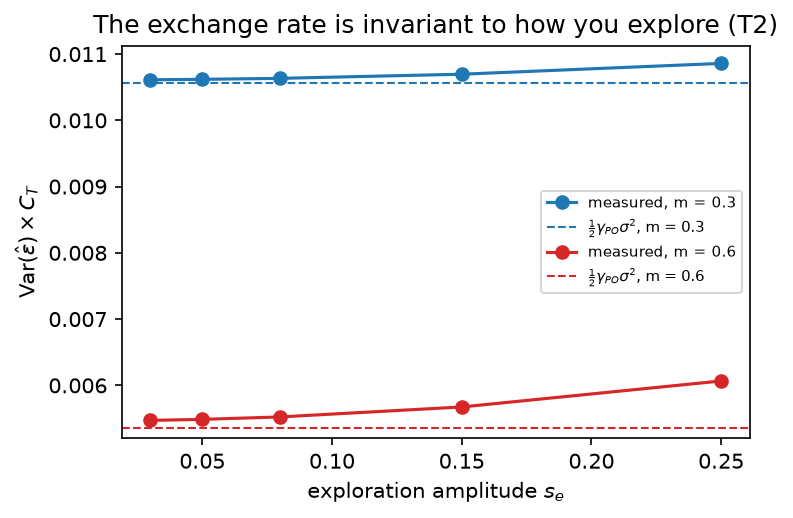
\includegraphics[width=\textwidth]{fig1_exchange_rate.png}
\end{minipage}\hspace{0.03\textwidth}
\begin{minipage}{0.335\textwidth}
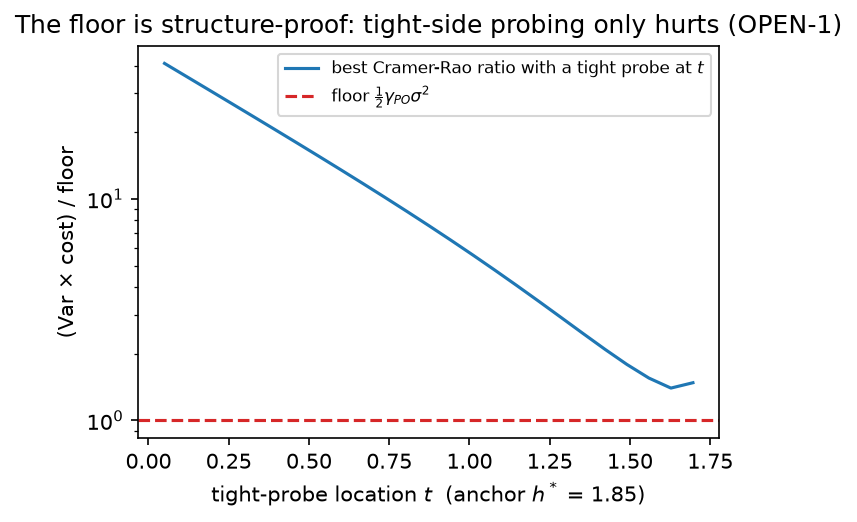
\includegraphics[width=\textwidth]{fig6_open1.png}
\end{minipage}
\caption{\textbf{Left:} the exchange rate of Theorem \ref{thm:exchange}.
Measured $\Var(\hat\eps)\times C_T$ against exploration amplitude at two
contraction moduli, flat on the invariant (dashed). \textbf{Right:} the
search that produced the false verdict. Best Cram\'er--Rao ratio with one
tight probe at $t$, over the coarse weight grid with $w \ge 0.05$. On this
family tight probes are monotonically worse, which is what we believed. The
counterexample lives outside it: probe weight $3\times 10^{-4}$, inside an
asymmetric cluster the search never generated.\label{fig:two}}
\end{figure}

\textbf{Why the first search missed it, exactly.} Two gaps, both now
identified. The scan's weight grid never went below $0.05$, and the violating
probe carries $3\times 10^{-4}$. The random search did generate distant
probes, but always alongside a symmetric near-anchor pair, and
symmetric-pair-plus-far-probe families never break the floor: their ratio
approaches $1$ from above as the probe weight vanishes. The violation
requires the asymmetric cluster. The earlier verdict was therefore neither
noise nor a coding error. It was a correct summary of a search space that
happened to exclude the answer, and nothing inside that search could have
revealed the exclusion.

\begin{theorem}[Structure-proofness, exact reach; T9]
\label{thm:reach}
(i) Every estimable design supported in $[\hstar - 2/c, \infty)$ satisfies
$R(\mu) \ge 1$, strictly except on one two-point configuration, and
$\inf_\mu R(\mu) = 1$. Within reach, knowing the family cannot beat the
floor. (ii) The reach is exact: the four-point witness above attains
$R = 0.8517$.
\end{theorem}

\textbf{The corrected result explains itself.} The two-sided statement says
something the one-sided belief did not. Structure-proofness is an
ignorance-of-curvature phenomenon with an exactly known extent. A design
reaching far enough below the anchor learns the curvature parameter $c$
cheaply enough to bank that cheapness rather than pay for it, and the floor
stops binding. Two boundary checks confirm the reading. With $c$ known a
priori, so that the ignorance is gone, the floor breaks outright and keeps
falling with no limit the scan reaches ($R = 0.3002$ at probe $t = 1.0$,
$0.0425$ at $t = 0.05$, $0.0348$ and still decreasing at $t = 0.001$). And the
reach is exactly where a trust-region agent can deploy, since its clip is
$r \le 0.8 < 2/c = 1.333$: the constraint that keeps it safe is the one that
keeps its lower bound valid. That was read off the corrected theorem, not
designed.

\section{The loop, and what it generalizes to}
\label{sec:loop}

One episode is an anecdote. This section gives the sample it sits in and
states what that sample supports.

\textbf{The division of labour.} Automated: numerical evaluation of every
closed form against a simulation, at tolerances declared before the run;
adversarial search over designs; high-precision arithmetic on frozen
candidates; regression checking on every push. Not automated: every proof in
this work, every choice of what to conjecture, and the decision to search
below the reach. The machine in this loop is a fast, tireless, uncreative
referee. It never proposed a theorem. It refuted several, and in the eleventh
case only after a human argument told it where to look.

\textbf{Eleven pivots, three of them the same shape.} Measurement forced
eleven changes to written-down claims, and three repeat the lead story at
smaller scale. In E1, a saturation cap derived without noise failed by a
factor of four against the noisy pipeline; the gap was a missing term, since
retraining on noisy observations adds a stationary excitation floor of
$(\sigma/\gamma)^2/(1-m^2)$ per step, now itself verified within $0.2$ to
$6.4$ percent. In E5, an injected misspecification $a e^{-2ch}$ had decayed
to about $10^{-3}$ by the operating point, so the anchored fit correctly
never saw it; replacing it with a linear leak the family cannot represent
produced the crossover the theory predicts. In E7, a claimed threefold
advantage for shaped exploration collapsed to parity once the comparison arm
was funded with the same energy, the unshaped arm having been given $r^2/3$
per step against the design's $2r^2/3$; the corrected claim is sharper, since
the identification cliff is a support and amplitude phenomenon rather than a
shape phenomenon. In each case the replacement was a stronger statement than
the claim it displaced.

\textbf{What the sample supports.} A modest and specific thing: on this
project, numerical falsification was cheap and frequent, and it improved
claims rather than merely deleting them. It supports no claim about proof
automation, about other areas of mathematics, or about what happens without a
person deciding where to look. The eleventh pivot needed a proof to produce
the region, and no further search inside the original space would have found
it.

\textbf{The infrastructure, which is the transferable part.} A theorem
register lists all 26 results with per-result proof status, distinguishing
proved, proved for a stated class, and proved conditional on a hypothesis, so
a numerically supported conjecture cannot quietly be cited as a theorem. A
preregistered harness compares each measurement to a closed form at a
tolerance fixed before the run; the state is 36 rows with 0 failures, one of
them a deliberately out-of-scope cell reported as drift rather than excused.
A derivation suite of 38 checks runs in continuous integration, and its first
runs falsified three drafted claims, one with the wrong predicted sign. Every
pivot is written into the code file where it occurred, which is why the
eleventh survives as a record and not as a memory.

\textbf{The honesty discipline is part of the contribution.} We report the
drift cell as drift. We label the sharp constant $\tfrac12$ in T4 as
numerically supported and open, since what is proved is the constant-factor
version. And we say plainly that our own written verdict of
structure-proofness was a search artifact. A record containing only successes
cannot calibrate how much to trust the next numerical verdict, which is the
only reason to keep one.

\textbf{Limitations.}\label{sec:limits} Theorem \ref{thm:exchange} is local
and its $o(1)$ is load-bearing: wide-side probing at finite amplitude
undercuts the identity, and the out-of-scope saturating cell drifts $+16$
percent. The value-budget floor T4 is proved only to within a factor of
$13.5$ of the conjectured constant. Theorem \ref{thm:reach}(ii) lives inside
the local-quadratic cost model, where under the true cost the same witness
has ratio $1.0112$, so the violation concerns the floor's own scope and not
the underlying market. Which below-reach designs violate it, and by how much
at most, is open. And this section rests on eleven pivots from one project by
one group, which is a sample and not a study.

\bibliographystyle{plainnat}
\bibliography{references}

\clearpage
\appendix

\section{Assumptions and statements}
\label{app:statements}

This appendix collects the standing assumptions and the formal statements of
every result the body refers to, and nothing else. Identifiers (L1, T2, T9,
and so on) are the register identifiers used throughout the supplementary
repository, so each statement here can be matched to its derivation
document, its proof, and its numerical checks. The register itself, with
per-result proof status, is \texttt{mlxor-derivations/THEOREMS.md}.

\subsection{Standing assumptions}

\textbf{A1} (local quadratic scope): $\Phi$ is $C^3$ and strongly concave on
the operating interval, with expansions taken at $\hstar$ and third-order
remainder bounded by $L_3 = \sup|\Phi'''|$.
\textbf{A2} (exploration class): all policies are non-anticipating; A2-sym
adds $\E[u_t \mid \mathcal{F}_t] = 0$, A2-adaptive is
unrestricted, and costs are measured from the certainty-equivalent anchor.
\textbf{A3} (noise exogeneity): the observation noise $\zeta_t$ is i.i.d.,
mean zero, variance $\sigma^2$, independent of $\mathcal{F}_t$. A3$'$ relaxes
this to a feedback channel with gain $\phi$.
\textbf{A4} (trust region): $|\dev_t| \le r$ pathwise.
\textbf{A5} (stationary scale): $S_T = \Theta(T)$.
\textbf{A6} (stable base loop): the retraining modulus satisfies $m < 1$.

The local dynamics are $\dev_{t+1} = -m\,\dev_t + u_t$ with
$\dev_t = h_t - \hstar$, observations
$\tau_t = \tau(\hstar) - \eps\,\dev_t + \zeta_t$, and $\Phi$ satisfying
$\Phi'(\hstar) = \delta_0$ and $-\Phi'' = \gpo$ at the operating point.
$\Sxx$ denotes the centered design energy $\sum_{t\le T}(\dev_t -
\bar\dev)^2$.

\subsection{The exchange rate and its floors}

\begin{lemma}[Cost equivalence; L1]
\label{lem:cost}
Under A1--A3 with conditionally symmetric exploration, the expected
incremental performative cost satisfies
$C_T = \tfrac{1}{2}\gpo\,\E\!\big[\sum_{t\le T}\dev_t^2\big] + R_T$ with
$|R_T| \le \tfrac{L_3}{6}\,\E\sum_t |\dev_t|^3$, and the realized cost's
variance decomposes exactly as
$\Var(C_T^{\mathrm{real}}) = \delta_0^2\,\Var\!\big(\sum_t \dev_t\big)
+ \tfrac{\gpo^2}{4}\,\Var\!\big(\sum_t \dev_t^2\big)$
with vanishing cross term.
\end{lemma}

\begin{theorem}[Information saturation; T1]
\label{thm:sat}
With no deliberate exploration and $\rho(M)<1$, the total design energy of
the retraining trajectory equals $\dev_0^\top P\,\dev_0$, where $P$ solves
the discrete Lyapunov equation $P = I + M^\top P M$. Consequently the Fisher
information for the response Jacobian is bounded in every direction,
uniformly in the horizon. In the scalar case the cap is
$\dev_0^2/(1-m^2)$, strictly increasing in $m$: a fast-contracting loop
reveals least about its own performativity (C1.1). Under the noisy feedback
channel A3$'$ the trajectory additionally carries a stationary excitation
floor of $(\sigma/\gamma)^2/(1-m^2)$ per step.
\end{theorem}

The body's Theorem \ref{thm:exchange} is the asymptotic form of the following
pathwise identity, which is what is proved in Appendix \ref{app:proofs}.

\begin{theorem}[The exchange rate, pathwise; T2]
\label{thm:t2exact}
Under A1, A2-sym, A3 and A6, in the stationary regime, on every realization,
\[
\Var(\hat\eps \mid \mathrm{design}) \times \tfrac{1}{2}\gpo \sum_{t\le T}
\dev_t^2 \;=\; \tfrac{1}{2}\,\gpo\,\sigma^2\Big(1 +
\tfrac{T\,\bar{\dev}^2}{\Sxx}\Big)
\;=\; \tfrac{1}{2}\,\gpo\,\sigma^2\,\big(1 + O_P(1/T)\big),
\]
independent of the exploration intensity, the horizon, and the modulus.
\end{theorem}

\begin{theorem}[Minimax lower bound, deviation budget; T3]
\label{thm:t3}
Over all non-anticipating exploration policies with
$\sum_{t\le T} \dev_t^2 \le D$ almost surely and all estimators, biased
included, the minimax risk over an interval of width $w$ satisfies
$\inf \sup_{\eps} \E[(\hat\eps - \eps)^2] \ge \sigma^2/(D + \sigma^2
(\pi/w)^2)$, so the exchange-rate product is a floor, attained with equality
by symmetric probing with least squares.
\end{theorem}

\begin{lemma}[Exploitation and information; L2]
\label{lem:l2}
For the symmetric two-point response family with half-width $\delta$ and any
non-anticipating policy under the certainty-equivalent anchor,
$\E[\mathrm{gain}_T] \le g_1\,\delta^{3/2}\,T^{1/2}\,(\E S_T)^{3/4}
\sigma^{-1/2}$ with $g_1 = \beta\,|\hstar - \psi|$, via the identity
$\E|\E[s\mid\mathcal{F}_t]| = \TV(P^+_t, P^-_t)$ and Pinsker's inequality.
At the minimax scale this is an $O(T^{-1/2})$ fraction of the exploration
cost.
\end{lemma}

\begin{theorem}[Minimax lower bound, value budget; T4]
\label{thm:t4}
Under stationary-scale exploration and the certainty-equivalent anchor, for
every non-anticipating policy and every estimator,
$\sup \Var(\hat\eps)\times C_T \ge \gpo\,\sigma^2/27\,(1 - O(T^{-1/2}))$,
the supremum over the two-point response family at the minimax scale, the
constant arising from a Le Cam reduction optimized at $c = 2/3$. The sharp
constant $\tfrac{1}{2}$, against which no simulated policy fell by more than
Monte Carlo error, is conjectured and is part of the open problem OPEN-1. It
is not proved here or anywhere in the repository.
\end{theorem}

\subsection{Design and certification}

\begin{theorem}[A-optimal exploration; T5a]
\label{thm:t5a}
Under the value budget $\tr(\Gpo M) \le B$ on the exploration second moment
$M$, the A-optimal design is $M^{*} = (B/\tr\,\Gpo^{1/2})\,\Gpo^{-1/2}$,
with value $(\tr\,\Gpo^{1/2})^2/B$: explore where the objective is flat.
\end{theorem}

\begin{corollary}[Price of isotropic jitter; C5.1]
\label{cor:c51}
Isotropic exploration at matched budget overpays the A-optimal design by
exactly the curvature-dispersion factor
$F = d\,\tr(\Gpo)/(\tr\,\Gpo^{1/2})^2 \ge 1$, with equality if and only if
all curvature directions are equal.
\end{corollary}

\begin{theorem}[Chebyshev unidentifiability; T6]
\label{thm:t6}
The sensitivity system of the structural family
$\tau(h) = C_0 + C_1 e^{-ch}$ is an extended Chebyshev system. Any design
with fewer than three support points has singular Fisher information, and
since noiseless retraining trajectories have at most two effective support
points, no retraining trajectory at any modulus identifies the response
curvature $c$.
\end{theorem}

\begin{theorem}[Anchoring crossover; T7]
\label{thm:t7}
Under the value budget $B$ and horizon $T$, the budget-and-horizon-optimal
nonparametric secant estimator has
$\mathrm{MSE}_{\mathrm{np}} = \gpo\sigma^2/(2B) + (\tau'''(\hstar)/6)^2
(2B/(\gpo T))^2$, so anchoring to a structural family with misspecification
$\delta_{\mathrm{mis}}$ wins, to leading order, if and only if
$\delta_{\mathrm{mis}} < |\tau'''(\hstar)|\,B/(3\,\gpo\,T)$.
\end{theorem}

\begin{lemma}[Perturbed modulus; L4]
\label{lem:l4}
If the corrected update uses an estimated response with $C^1$ error $e$, the
closed-loop modulus satisfies $|\hat\rho - \rho| \le \eta\,\beta\,
(\|e\|_\infty + |\hstar-\psi|\,\|e'\|_\infty)$.
\end{lemma}

\begin{proposition}[Safety under pessimism; P7.1]
\label{prop:p71}
Given an anytime-valid confidence sequence for the response parameters at
level $1-\delta$, the pessimism rule, which keeps the worst-case modulus over
the confidence set below $1 - c_{\mathrm{margin}}$ and freezes the correction
otherwise, keeps the realized modulus within the margin for all $t$
simultaneously with probability at least $1-\delta$. The result is
conditional on the validity of the confidence sequence, and the register
records it as such.
\end{proposition}

\subsection{Structure-proofness}

\begin{theorem}[Structure-proofness of the floor, exact reach; T9]
\label{thm:t9full}
Fix the structural family $\tau_\theta(h) = C_0 + C_1 e^{-ch}$
($C_1 > 0$, $c > 0$), the anchor $\hstar > 0$, the sensitivity
$s(h) = \partial_\theta \tau_\theta(h)$, and the estimand gradient
$g = \partial_\theta\,\eps(\hstar) = -s'(\hstar)$. For a finitely supported
design $\mu$ define the normalized Cram\'er--Rao product
\[
R(\mu) \;=\; \big(g^\top M(\mu)^{-1} g\big)\!\int (h - \hstar)^2\,
d\mu, \qquad M(\mu) = \int s\,s^\top d\mu,
\]
so that $R(\mu) \ge 1$ states that the family-knowing Cram\'er--Rao product
$\Var(\hat\eps)\times C_T$ is at least the exchange-rate floor
$\tfrac{1}{2}\gpo\sigma^2$ under the local-quadratic (A1) cost, for unbiased
estimators and, in the local-asymptotic-minimax sense, for all regular
estimators.
(i) \emph{Within reach the floor is structure-proof:} if
$\mathrm{supp}(\mu) \subset [\hstar - 2/c,\,\infty)$, then either
$\eps(\hstar)$ is not estimable under $\mu$, in which case the bound is
infinite, or $R(\mu) \ge 1$, strictly whenever $\mu$ places mass off the two
equality points $\{\hstar,\ \hstar - 2/c\}$; and $\inf_\mu R(\mu) = 1$,
approached but not attained by symmetric three-point designs collapsing at
$\hstar$. In particular the floor binds on every trust-region design with
$r \le 2/c$.
(ii) \emph{The reach is exact:} the pointwise domination underlying (i) fails
strictly below $\hstar - 2/c$, and an explicit four-point design with a
single below-reach probe of weight $3\times 10^{-4}$ attains $R = 0.8517$,
computer-verified at 50-digit precision as check V9.2.
\end{theorem}


\section{Proofs}
\label{app:proofs}

This appendix proves the two results the body argues from: the exchange
rate of Theorem \ref{thm:exchange}, whose exact pathwise form is stated as
Theorem \ref{thm:t2exact}, and the two-sided structure-proofness result of
Theorem \ref{thm:reach}, stated in full as Theorem \ref{thm:t9full}. Both
proofs are
reproduced from the derivation repository without change; the check
identifiers V2.1 and V9.1 to V9.4 refer to its verification suite. Proofs of
the remaining statements in Appendix \ref{app:statements} are in that
repository and are not reproduced here.

\subsection*{The cost-equivalence lemma}

\begin{proof}[Proof of Lemma L1 (cost equivalence)]
Taylor's theorem with Lagrange remainder gives, for each $t$,
\[
\Phi(\hstar) - \Phi(h_t)
 = -\delta_0\,\dev_t + \tfrac{1}{2}\gpo\,\dev_t^2 + r_t,
 \qquad |r_t| \le \tfrac{L_3}{6}\,|\dev_t|^3,
\]
with $L_3 = \sup |\Phi'''|$ on the operating interval. Summing over
$t \le T$ and taking expectations, it remains to show
$\E[\sum_t \dev_t] = 0$ under A2-sym. The recursion gives
$\E[\dev_{t+1} \mid \mathcal{F}_t] = -m\,\dev_t + \E[u_t \mid \mathcal{F}_t]
= -m\,\dev_t$, so $\E[\dev_{t+1}] = -m\,\E[\dev_t]$ by the tower property,
and $\E[\dev_t] = (-m)^t\,\E[\dev_0] = 0$ when the loop starts at the
operating point or in the stationary regime. The quadratic term contributes
$\tfrac{1}{2}\gpo\,\E[\sum_t \dev_t^2]$, which is the claim.

For the variance decomposition, write the realized cost (net of the cubic
remainder) as $C = -\delta_0 X + \tfrac{1}{2}\gpo Y$ with
$X = \sum_t \dev_t$, $Y = \sum_t \dev_t^2$. Then
$\Var(C) = \delta_0^2 \Var(X) + \tfrac{\gpo^2}{4}\Var(Y)
- \delta_0\gpo\,\Cov(X, Y)$. Under Gaussian innovations the vector
$(\dev_1,\dots,\dev_T)$ is jointly Gaussian with mean zero, and every third
moment of a zero-mean Gaussian vector vanishes; since
$\Cov(X,Y) = \sum_{t,s}\E[\dev_t\,\dev_s^2]$ is a sum of third moments, it is
zero. (For non-Gaussian symmetric innovations the same conclusion follows
from the sign symmetry $\dev \mapsto -\dev$ of the stationary law.)
Verified: V0.1--V0.3, including the necessity check that an asymmetric rule
breaks the expectation identity by exactly $-\delta_0\,\E[\sum_t \dev_t]$.
\end{proof}

\subsection*{The exchange rate}

\begin{proof}[Proof of Theorem T2 (pathwise exchange rate)]
Under A3, conditionally on the design $\{\dev_t\}$ the observations are
independent with means linear in $\eps$ and variance $\sigma^2$, so the
least-squares slope has conditional variance
$\Var(\hat\eps \mid \mathrm{design}) = \sigma^2/\Sxx$ (Gauss--Markov).
Multiplying by the quadratic cost $\tfrac{1}{2}\gpo \sum_t \dev_t^2$ and
using $\sum_t \dev_t^2 = \Sxx + T\bar\dev^2$ gives the displayed identity
exactly, on every realization. In the stationary regime
$\bar\dev = O_P(T^{-1/2})$ by the stationary long-run variance $\Var(\sum_{t\le T}\dev_t) = T v (1-m)/(1+m)(1+o(1))$, while
$\Sxx/T \to v$ a.s., so $T\bar\dev^2/\Sxx = O_P(1/T)$. Verified: V2.1
(machine precision).
\end{proof}


\subsection*{Structure-proofness, and the exactness of the reach}

\begin{proof}[Proof of Theorem T9 (structure-proofness within reach)]
Write $x = h - \hstar$, $d(h) = x$, and
$V = \mathrm{span}\{1,\, e^{-ch},\, h e^{-ch}\}$, the span of the
components of $s$ (a bijective correspondence $u \leftrightarrow
\phi_u = u^\top s$ between $\mathbb{R}^3$ and $V$, since $C_1 \neq 0$).
Differentiating $s$ gives
$s'(h) = (0,\, -c e^{-ch},\, C_1 e^{-ch}(ch - 1))^\top$, so
$g = -s'(\hstar)$ componentwise, which is the stated estimand gradient.

\emph{Step 1: one-dimensional reduction.} For $M(\mu) \succ 0$ the
generalized Rayleigh identity gives
\[
g^\top M(\mu)^{-1} g
 = \sup_{u \neq 0} \frac{(u^\top g)^2}{u^\top M(\mu)\, u}
 = \sup_{\phi \in V} \frac{\phi'(\hstar)^2}{\int \phi^2\, d\mu}
 = \Big(\inf\big\{ \textstyle\int \phi^2\, d\mu :
   \phi \in V,\ \phi'(\hstar) = 1 \big\}\Big)^{-1},
\]
using $u^\top M u = \int \phi_u^2\, d\mu$ and $u^\top g =
-\phi_u'(\hstar)$ (the sign is lost in the square). Hence
\[
R(\mu) \;=\; \frac{\int d^2\, d\mu}
{\inf\{\int \phi^2 d\mu : \phi \in V,\ \phi'(\hstar) = 1\}}.
\]

\emph{Step 2: the candidate and its pointwise domination.} Let
\[
\phi_0(h) \;=\; \frac{2}{c} - e^{-cx}\Big(\frac{2}{c} + x\Big)
 \;=\; \frac{2}{c}\cdot 1
 \;-\; e^{c\hstar}\Big(\frac{2}{c} - \hstar\Big)\, e^{-ch}
 \;-\; e^{c\hstar}\, \big(h e^{-ch}\big) \;\in\; V,
\]
the unique element of $V$ with 2-jet $(0, 1, 0)$ at $\hstar$ (the
2-jet map is invertible on $V$: in the basis $\{1, e^{-ch}, h e^{-ch}\}$
its determinant is $c^2 e^{-2c\hstar} \neq 0$); the expansion is
$\phi_0(x) = x - (c^2/6)\,x^3 + O(x^4)$. Writing
$f(x) = \tfrac{2}{c} - e^{-cx}(\tfrac{2}{c} + x)$ we claim
\[
|f(x)| \le |x| \quad \text{for all } x \ge -2/c,
\qquad \text{with equality iff } x \in \{0, -2/c\},
\]
and $|f(x)| > |x|$ strictly for every $x < -2/c$. Indeed:
(a)~$v(x) = f(x) - x$ has $v(0) = 0$ and
$v'(x) = e^{-cx}(1 + cx) - 1 < 0$ for $x \neq 0$ (since $1 + t < e^t$
for $t = cx \neq 0$); $v' \le 0$ with equality only at the isolated
point $0$ makes $v$ strictly decreasing on $\mathbb{R}$, so $f > x$ on
$x < 0$ and $f < x$ on $x > 0$.
(b)~$f(0) = 0$ and $f'(x) = e^{-cx}(1 + cx) > 0$ for $x \ge 0$, so
$f \ge 0$ on $[0, \infty)$ and, with (a), $0 \le f \le x$ there.
(c)~$q(x) = f(x) + x$ has $q(-2/c) = 0 = q(0)$ and
$q'(x) = e^{-cx}(1 + cx) + 1$, where $r(x) = e^{-cx}(1 + cx)$ is
strictly increasing on $x < 0$ ($r'(x) = -c^2 x\, e^{-cx} > 0$) from
$r(-2/c) = -e^2 < -1$ to $r(0) = 1$; so $q'$ changes sign exactly once
on $(-2/c, 0)$, from negative to positive, and $q \le 0$ there with
equality only at the endpoints; with (a) ($f \ge x$, equality only at
$0$) this gives $x \le f \le -x$ on $[-2/c, 0]$.
(d)~For $x < -2/c$, $r(x) < -e^2$ gives $q' < 0$, so moving left from
$-2/c$ the function $q$ increases above $0$: $f(x) > -x = |x| > 0$,
and in fact $f(x) = 2/c + e^{c|x|}(|x| - 2/c)$ grows exponentially.

\emph{Step 3: the bound.} If $\mathrm{supp}(\mu) \subset
[\hstar - 2/c, \infty)$, Step 2 gives $\int \phi_0^2\, d\mu \le \int
d^2\, d\mu$, so by Step 1, $R(\mu) \ge \int d^2 d\mu / \int \phi_0^2
d\mu \ge 1$. Strictness: equality in Step 2 holds only at
$x \in \{0, -2/c\}$, so any $\mu$ placing positive mass off
$\{\hstar, \hstar - 2/c\}$ (in particular any with three distinct
support points) has $\int \phi_0^2 d\mu < \int d^2 d\mu$ and
$R(\mu) > 1$. If $M(\mu)$ is singular, two cases:
$g \notin \mathrm{range}\,M(\mu)$ makes $\eps(\hstar)$ non-estimable
(infinite bound); $g \in \mathrm{range}\,M(\mu)$, which does occur for
special two-point designs (a one-parameter family of in-reach pairs;
their finite pseudo-inverse products were checked to obey the bound,
e.g.\ $R = 1.063$ at the pair $\{1.627, 2.127\}$), keeps
the sup-representation valid over $\{u : u^\top M u > 0\}$, and
$\int \phi_0^2 d\mu = 0$ would put $u_0 \in \mathrm{null}\, M$ with
$u_0^\top g = -1 \neq 0$, contradicting $g \in \mathrm{range}\,M$; so
$\int \phi_0^2\, d\mu > 0$ and the bound goes through verbatim.
Throughout, the Cram\'er--Rao functional bounds unbiased estimation,
and all regular estimators in the local-asymptotic-minimax sense.

\emph{Step 4: the infimum is 1.} The Cram\'er--Rao functional is
invariant under $C^1$ reparametrization, and the 2-jet map
$\theta \mapsto (\tau_\theta(\hstar),\, \eps(\hstar),\,
\tau_\theta''(\hstar))$ is a local diffeomorphism: its Jacobian
$[\,s(\hstar)\ {-s'(\hstar)}\ s''(\hstar)\,]$ has determinant
$C_1 c^2 e^{-2c\hstar} \neq 0$ (direct computation; V9.4). In jet
coordinates $\eta$ the model reads $\tau = \eta_1 - \eta_2 x +
\tfrac{1}{2}\eta_3 x^2 + O(x^3)$ with sensitivity $\tilde s(x) =
(1, -x, x^2/2)^\top + O(x^3)$, and the estimand is $\eta_2$. For the
symmetric three-point design $\mu_\delta$ uniform on $\{\hstar -
\delta, \hstar, \hstar + \delta\}$, scale by $D = \mathrm{diag}(1,
\delta, \delta^2)$: $M_\eta(\mu_\delta) = D\,\hat H_\delta\, D$ with
$\hat H_\delta \to \hat H_0$ invertible (the exact quadratic-model
moment matrix), so $(M_\eta^{-1})_{22} = \delta^{-2}(\hat
H_\delta^{-1})_{22}$ and $R(\mu_\delta) \to R_{\mathrm{quad}}$. In
the exact quadratic model, for \emph{any} symmetric design (odd
moments $m_1 = m_3 = 0$), the $(2,2)$ cofactor gives
$(M_\eta^{-1})_{22} = 1/m_2$ and $R_{\mathrm{quad}} = m_2 \cdot
(1/m_2) = 1$. Hence $R(\mu_\delta) \to 1$ (measured rate
$R(\mu_\delta) - 1 = O(\delta^2)$; V9.2), the infimum is 1, and by
Step 3 it is not attained.

\emph{Step 5: the reach is exact.} Below $\hstar - 2/c$ the
domination of Step 2 fails strictly, and the failure is realized by a
design, not only by the candidate: the frozen four-point witness
(support $\{1.8726, 1.8665, 1.3073, 0.0500\}$, weights
$\{0.003329, 0.955702, 0.040697, 0.000272\}$ after normalization, in
the register market $c = 1.5$, frozen anchor $\hstar = 1.8461$) has
$R = 0.851650\ldots$, verified at 50-digit precision (mpmath) and
reproduced in float64 by \texttt{run\_open1.py} (V9.2). All its
support except the probe at $0.05$ lies within reach: one
vanishing-weight below-reach probe breaks the floor. Symmetric
pair-plus-far-probe families do \emph{not} break it (their ratio
approaches 1 from above as the probe weight vanishes); the violation
requires the asymmetric cluster, which is why coarse searches missed
it. Verified: V9.1--V9.4.
\end{proof}



\clearpage
\section{Verification rows}
\label{app:table}

\begin{table}[H]
\centering
\small
\caption{Selected rows from the preregistered check harness. The full table
(36 rows, 0 FAIL), all seeds, tolerances, and code are in the supplementary
repository. The drift row is a deliberately out-of-scope cell, measured and
reported rather than excused.}
\label{tab:results}
\begin{tabular}{@{}llll@{}}
\toprule
Claim (register) & Measured & Predicted & \\
\midrule
Exchange rate, $m{=}0.3$, two amplitudes (T2) & $0.01062,\ 0.01070$ & $0.01056$ & pass \\
Exchange rate, $m{=}0.6$, two amplitudes (T2) & $0.00549,\ 0.00569$ & $0.00535$ & pass \\
Saturating environment (outside A1) & $+16\%$ over rate & out of scope & drift \\
Feedback floor, $m{=}0.3/0.6/0.85$ (T1 corollary) & within $0.2$--$6.4\%$ & $(\sigma/\gamma)^2/(1{-}m^2)$ & pass \\
Design arm $\mathrm{sd}(\hat c)$; jitter/design ratio (T6) & $0.234$; $7.8\times$ & Fisher $0.248$; $\ge 3$ & pass \\
Certified agent reaches $\hpo$; trust region (L4) & $1.258$; $0$ violations & $1.296$; $0$ & pass \\
Isotropic/A-optimal risk ratio, $d{=}8$ (T5a) & $1.529$ & $F = 1.506$ & pass \\
Nonparametric MSE at $(B,T)$ optimum (T7) & $0.0132$ & $0.0123$ & pass \\
Second economy, 4 cells (T2, exact in LQ); agent & $0.384,\ 0.192$; $12.65$ & $0.384,\ 0.192$; $12.5$ & pass \\
Multi-book shaped/isotropic steady-state risk (T5a) & $1.20$ (flat control $1.00$) & $>1.15$ ($\approx 1$) & pass \\
Real-data calibration port, 10 cells & $10/10$ reproduce & within $0.8\%$ & pass \\
Within-reach min CR ratio; witness beyond (T9) & $1.0005$; $0.8517$ & $\ge 1$; $< 1$ & pass \\
\bottomrule
\end{tabular}
\end{table}

\section{Reproducibility and scope of this version}
\label{app:repro}

\textbf{What ships.} The supplementary repository contains the derivation
documents and the theorem register (26 results, 38 numerical derivation
checks), the simulation pipeline (environments, estimators, designs, agents,
baselines; 36 measured-versus-predicted rows; 9 unit tests), the real-data
port with its 10-cell validation, and the eleven-pivot record in the pipeline
README. Both verification suites run in continuous integration on every push
in the project repository; the two workflow files are not part of this
anonymized copy. The structural market used throughout, and the corporate-bond
calibration behind the real-data row of Table \ref{tab:results}, are those of REFLEX
\citep{reflex2026}, on which this work builds. All results are deterministic from seeds, numpy-only, and CPU-only.
Reported final errors are 300-step tail averages over the deployed path,
stable within $0.01$ under horizon perturbation, with a worst measured spread
of $0.0062$.

\textbf{What is stated here but not proved here.} This version proves
Theorem \ref{thm:exchange} and Theorem \ref{thm:reach}, the two results the
body argues from. The minimax floors and the design and certification
results (T3, T4, T5a, C5.1, T6, T7, L4, P7.1) are stated in Appendix
\ref{app:statements} and proved in the supplementary repository, in
\texttt{mlxor-derivations/latex/proofs.tex} and the corresponding derivation
documents, with the register recording each result's proof status.

\textbf{Provenance of the numbers.} Every quantity in the body and in Table
\ref{tab:results} is copied from a committed artifact:
\texttt{results/RESULTS.md} for the harness rows, \texttt{results/OPEN1.md}
for the reach, the witness, and the search history,
\texttt{results/REALDATA.md} for the calibration port,
\texttt{results/STABILITY.md} for the tail-average stability,
\texttt{results/full\_run.log} for quantities not surfaced in the summary
tables, and \texttt{THEOREMS.md} for the register. The runs behind them were
executed and recorded on 1 September 2026. This version re-narrates them and
does not re-run them, since none of its changes touch their inputs.

\end{document}
